\documentclass[herrin-thesis.tex]{subfiles}
\begin{document}

\chapter{Data Collection and Processing}
\label{ch:data}

\section{Signal Readout}
\begin{figure}
\centering
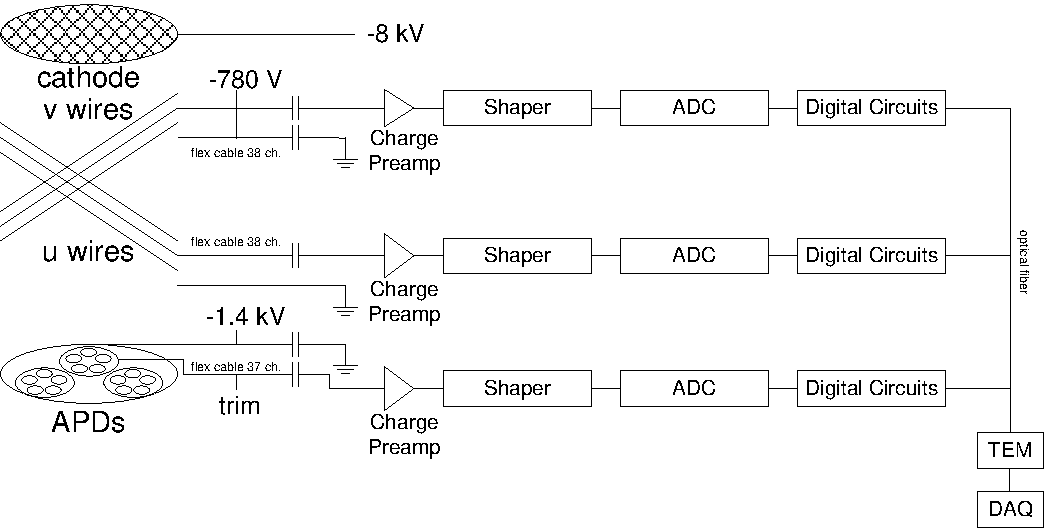
\includegraphics[width=\textwidth]{./figures/data_simplified_electronics.pdf}
\caption[The EXO-200 electronics]{A simplified schematic of the EXO-200 electronics. The ionization and scintillation signals are read out through long flex cables. The signals are shaped, digitized, and passed to the Trigger Event Module (TEM), which passes the data to the DAQ computers for recording when signals are detected.}
\label{fig:data_simplified_electronics}
\end{figure}

\Cref{fig:data_electronics_schematic} shows a simplified schematic for the EXO-200 electronics. The APD signals and the ionization inductions and collection signals are read out through long flex cables. The long cables separate the electronics from the TPC, removing the need for cryogenic and low-radioactivity components. After passing through a preamplifier, the signals are fed through shaping circuits and are then digitized at a rate of \SI{1}{\MHz}. The shaping circuits for the APDs consist of \todo{Fill in.}. The ionization readout passes through \todo{This too.}.

After digitization, the Trigger Event Module (TEM) monitors the signals to select interesting events. Due to the low radioactive backgrounds in EXO-200, and the relatively slow rate of \twonu, this trigger is extremely permissive. It is 100\% efficient at triggering on events that deposit more that \todo{Look up} in the liquid xenon. The average trigger rate during routine data taking is approximately \SI{8}{\mHz}. Additionally, the trigger is forced to fire every \SI{0.1}{\s} in order to ensure the DAQ system is correctly recording events and to provide a measurement of detector live time.

\section{Signal Reconstruction}

\section{Corrections}
\subsection{Gain Corrections}
\subsection{Shielding Grid Corrections}
\subsection{Electron Lifetime Corrections}
\subsection{Light Collection Efficiency Corrections}

\section{Calibration}

\section{Data Quality Cuts}

\end{document}
